% ==========================================
% BAB V IMPLEMENTASI
% ==========================================
\cleardoublepage
\chapter{IMPLEMENTASI SISTEM REKOMENDASI MODUL \emph{PEOPLE-TO-PROJECT}}
\label{chap:implementasi}

% ==========================================
\section{Deskripsi Implementasi}

Bab ini menjelaskan hasil implementasi modul \emph{People-to-Project} pada aplikasi Platform Kolaborasi Mahasiswa berdasarkan hasil perancangan pada bab sebelumnya. Implementasi modul ini mencakup pengembangan aplikasi \emph{client} berbasis \emph{Flutter} yang berjalan pada perangkat \emph{Android}, serta pemanfaatan layanan \emph{backend} bersama yang telah disepakati ketiga anggota tim, yaitu \emph{REST API} berbasis \emph{Express.js} dengan \emph{Prisma} sebagai \emph{Object-Relational Mapping}, dan basis data \emph{PostgreSQL} pada platform \emph{Railway}.

Komunikasi antara aplikasi \emph{client} dan \emph{Application Server} dilakukan melalui protokol HTTPS dengan format data JSON, sedangkan logika pencocokan \emph{Affinity Based Matching} dan perhitungan skor keseimbangan tim berbasis \emph{Belbin} dijalankan pada sisi \emph{server} melalui komponen \emph{AffinityEngine}, sejalan dengan prinsip \emph{thin client} \autocite{sommerville2016} agar beban komputasi tidak membebani perangkat \emph{mobile} pengguna.

Implementasi modul \emph{People-to-Project} mencakup sebelas \emph{use case} sebagaimana telah dirancang pada Bab Perancangan, mulai dari autentikasi pengguna (\emph{Register}, \emph{Login}, \emph{Logout}), pengelolaan profil kolaboratif, pencocokan rekomendasi melalui \emph{AffinityEngine}, penelusuran \emph{feed} dan detail kegiatan kolaboratif, pendaftaran ke kegiatan kolaboratif, hingga pembuatan kegiatan dan pemrosesan pendaftar oleh pembuat kegiatan. Rincian lingkungan implementasi, status implementasi tiap \emph{use case}, pemetaan antarmuka, serta algoritma \emph{AffinityEngine} yang diimplementasikan dijelaskan pada subbab-subbab berikut.

Perlu ditegaskan bahwa perangkat lunak yang dihasilkan pada tahap ini berstatus sebagai prototipe dalam konteks pengerjaan Tugas Akhir, bukan produk siap produksi. Hal ini sejalan dengan batasan yang telah dinyatakan pada Bab Perancangan, yaitu \emph{deployment server} menggunakan layanan \emph{cloud} seperti \emph{Railway} untuk keperluan pengembangan prototipe, sementara pengujian \emph{client} dilakukan menggunakan \emph{Android emulator} dan perangkat fisik. Dengan demikian, cakupan fitur, performa, dan skala pengujian pada bab ini merepresentasikan kondisi prototipe, bukan kondisi operasional penuh.

% ==========================================
\section{Lingkungan Implementasi}

Lingkungan implementasi yang digunakan dalam pengembangan modul \emph{People-to-Project}, mengacu pada \emph{deployment diagram} yang telah dirancang pada Bab Perancangan, disajikan pada Tabel~\ref{tab:lingkungan-impl}.

\begin{longtable}{p{5cm} >{\raggedright\arraybackslash}p{\dimexpr\linewidth-5cm-4\tabcolsep\relax}}
  \caption{Lingkungan Implementasi Modul \emph{People-to-Project}}
  \label{tab:lingkungan-impl} \\
  \toprule
    \textbf{Lingkungan} & \textbf{Keterangan} \\
  \midrule
  \endfirsthead
  \multicolumn{2}{l}{\small\textit{Tabel~\ref{tab:lingkungan-impl} Lingkungan Implementasi Modul \emph{People-to-Project} (lanjutan)}} \\
  \toprule
    \textbf{Lingkungan} & \textbf{Keterangan} \\
  \midrule
  \endhead
  \bottomrule
  \multicolumn{2}{r}{\textit{Bersambung ke halaman berikutnya.}} \\
  \endfoot
  \bottomrule
  \endlastfoot
    \emph{Development Tools} & \emph{Visual Studio Code} \\
    \midrule
    Sistem Operasi & \emph{Windows} \\
    \midrule
    Bahasa Pemrograman & \emph{Dart} dan \emph{JavaScript} \\
    \midrule
    \emph{Framework Client} & \emph{Flutter} (perangkat \emph{mobile Android}, artefak \emph{.apk}) \\
    \midrule
    \emph{Backend}/API & \emph{Express.js} dengan \emph{Prisma} (\emph{REST API}) \\
    \midrule
    DBMS & \emph{PostgreSQL} \\
    \midrule
    \emph{Hosting} Aplikasi \emph{Server} dan Basis Data & \emph{Railway} \\
    \midrule
    Protokol Komunikasi \emph{Client-Server} & HTTPS, format data \emph{REST API} (JSON) \\
\end{longtable}

% ==========================================
\section{Batasan Implementasi}

Implementasi modul \emph{People-to-Project} pada tugas akhir ini dilakukan dalam lingkup prototipe sehingga terdapat sejumlah batasan yang perlu diperhatikan dalam membaca hasil implementasi dan pengujian pada bab ini.

\begin{enumerate}

  \item Algoritma pencocokan berbasis aturan, bukan \emph{machine learning}. Bobot diturunkan dari survei menggunakan ROC dan bersifat tetap; sistem tidak memiliki mekanisme \emph{feedback loop} atau pembaruan model dari data historis pengguna.

  \item Taksonomi \emph{skill}, minat, dan peran bersifat statis. Daftar atribut (12 tag \emph{skill}, 8 tag minat, 3 kategori peran) telah dikurasi sejak awal dan tidak dapat dikonfigurasi secara dinamis; penambahan atribut baru memerlukan perubahan kode.

  \item Pencocokan \emph{skill} dan minat berbasis \emph{exact string matching}. Fungsi \texttt{coverage()} mencocokkan tag secara \emph{case-insensitive exact match} tanpa pencocokan semantik atau sinonim sehingga perbedaan penulisan dari daftar tag baku tidak dikenali sebagai entitas yang sama.

  \item Skala pengalaman dan gaya kerja bersifat kategorikal terbatas. Level pengalaman dimodelkan dalam 3 tingkat ordinal dan gaya kerja dalam 2 kategori biner; nuansa di antara kategori tidak dimodelkan.

  \item Bobot kombinasi antarkomponen dan nilai ambang batas bersifat tetap. Rasio SkorAlgoritma1 dan SkorAlgoritma2 ditetapkan 50:50, dan nilai \emph{threshold feed} (0,3) serta ambang \emph{badge} (85\%/60\%/30\%) ditentukan berdasarkan pertimbangan desain, bukan hasil optimasi statistik atas data pengguna.

  \item \emph{AffinityEngine} bersifat \emph{pure function} dan terpisah dari lapisan data. Fungsi-fungsi di \texttt{affinityProject.ts} tidak mengakses basis data secara langsung; penanganan \emph{concurrency} saat banyak pengguna mendaftar ke kuota peran yang sama ditangani terpisah melalui transaksi basis data.

  \item Cakupan evaluasi kombinasi tingkat pengalaman belum menjangkau semua pasangan. Skenario AL04 menguji dua kasus representatif (selisih 1 dan 2 tingkat); seluruh 9 kombinasi pasangan (3 $\times$ 3) belum diuji satu per satu, meskipun prinsip perhitungannya identik.

  \item Platform terbatas pada aplikasi \emph{mobile Android} dan \emph{backend} prototipe. Aplikasi \emph{client} hanya tersedia dalam bentuk artefak \emph{.apk}; platform \emph{iOS} dan antarmuka \emph{web} tidak diimplementasikan, dan \emph{deployment} menggunakan \emph{Railway} untuk kebutuhan prototipe, bukan produksi berskala penuh.

  \item Ruang lingkup kategori atribut disesuaikan dengan konteks mahasiswa bidang teknologi informasi. Daftar tag \emph{skill}, minat, dan kategori peran dikurasi berdasarkan konteks kegiatan kolaboratif yang relevan bagi mahasiswa bidang teknologi, sejalan dengan profil responden survei yang juga berasal dari bidang yang sama. Atribut yang spesifik untuk bidang studi lain di luar teknologi informasi tidak tercakup dalam daftar ini.

\end{enumerate}

% ==========================================
\section{Implementasi \emph{Use Case}}

Daftar \emph{use case} modul \emph{People-to-Project} yang mengacu pada Tabel~\ref{tab:uc-traceability} pada Bab Perancangan, beserta status implementasinya, disajikan pada Tabel~\ref{tab:uc-impl}.

\begin{longtable}{p{0.4cm} p{1cm} p{4cm} p{2.5cm} >{\raggedright\arraybackslash}p{\dimexpr\linewidth-7.9cm-10\tabcolsep\relax}}
  \caption{Implementasi \emph{Use Case} Modul \emph{People-to-Project}}
  \label{tab:uc-impl} \\
  \toprule
    \textbf{No} & \textbf{Kode} & \textbf{Nama \emph{Use Case}} & \textbf{Status Implementasi} & \textbf{Nama File} \\
  \midrule
  \endfirsthead
  \multicolumn{5}{l}{\small\textit{Tabel~\ref{tab:uc-impl} Implementasi \emph{Use Case} Modul \emph{People-to-Project} (lanjutan)}} \\
  \toprule
    \textbf{No} & \textbf{Kode} & \textbf{Nama \emph{Use Case}} & \textbf{Status Implementasi} & \textbf{Nama File} \\
  \midrule
  \endhead
  \bottomrule
  \multicolumn{5}{r}{\textit{Bersambung ke halaman berikutnya.}} \\
  \endfoot
  \bottomrule
  \endlastfoot
    1 & UC01 & \emph{Register} & Ya & \texttt{auth.ts}, \texttt{auth.dart} \\
    \midrule
    2 & UC02 & \emph{Login} & Ya & \texttt{auth.ts}, \texttt{auth.dart} \\
    \midrule
    3 & UC03 & \emph{Logout} & Ya & \texttt{auth.ts}, \texttt{profil.dart} \\
    \midrule
    4 & UC04 & Mengelola Profil Kolaboratif & Ya & \texttt{general.ts}, \texttt{profil.dart} \\
    \midrule
    5 & UC05 & Melakukan Pencocokan Rekomendasi & Ya & \texttt{People\_to\_project.ts}, \texttt{peopleToProject.dart}, \texttt{affinityProject.ts} \\
    \midrule
    6 & UC06 & Melihat \emph{Feed} Rekomendasi Kegiatan & Ya & \texttt{People\_to\_project.ts}, \texttt{peopleToProject.dart}, \texttt{affinityProject.ts} \\
    \midrule
    7 & UC07 & Melihat Detail Kegiatan Kolaboratif & Ya & \texttt{People\_to\_project.ts}, \texttt{peopleToProject.dart} \\
    \midrule
    8 & UC08 & Mendaftar ke Kegiatan Kolaboratif & Ya & \texttt{People\_to\_project.ts}, \texttt{peopleToProject.dart} \\
    \midrule
    9 & UC09 & Membuat Kegiatan Kolaboratif & Ya & \texttt{People\_to\_project.ts}, \texttt{peopleToProject.dart} \\
    \midrule
    10 & UC10 & Melihat \emph{List} Pendaftar & Ya & \texttt{People\_to\_project.ts}, \texttt{peopleToProject.dart} \\
    \midrule
    11 & UC11 & Memproses Pendaftaran & Ya & \texttt{People\_to\_project.ts}, \texttt{peopleToProject.dart} \\
\end{longtable}

Seluruh \emph{use case} pada Tabel~\ref{tab:uc-impl} diimplementasikan dalam lingkup prototipe Tugas Akhir. Artinya, fungsi-fungsi tersebut diverifikasi melalui \emph{unit testing} dan pengujian fungsional sebagaimana dijelaskan pada metodologi, namun belum tentu mencakup penanganan skenario tepi (\emph{edge case}) secara menyeluruh maupun pengujian pada skala pengguna produksi.

% ==========================================
\section{Implementasi Antarmuka}

Daftar antarmuka yang diimplementasikan pada modul \emph{People-to-Project} beserta \emph{use case} yang dilayaninya disajikan pada Tabel~\ref{tab:antarmuka-impl}. Dokumentasi tampilan antarmuka tersebut disajikan pada Tabel~\ref{tab:antarmuka-visual}.

\begin{longtable}{p{1.5cm} p{7cm} >{\raggedright\arraybackslash}p{\dimexpr\linewidth-8.5cm-6\tabcolsep\relax}}
  \caption{Implementasi Antarmuka Modul \emph{People-to-Project}}
  \label{tab:antarmuka-impl} \\
  \toprule
    \textbf{Kode} & \textbf{Antarmuka} & \textbf{\emph{Use Case} Terkait} \\
  \midrule
  \endfirsthead
  \multicolumn{3}{l}{\small\textit{Tabel~\ref{tab:antarmuka-impl} Implementasi Antarmuka Modul \emph{People-to-Project} (lanjutan)}} \\
  \toprule
    \textbf{Kode} & \textbf{Antarmuka} & \textbf{\emph{Use Case} Terkait} \\
  \midrule
  \endhead
  \bottomrule
  \multicolumn{3}{r}{\textit{Bersambung ke halaman berikutnya.}} \\
  \endfoot
  \bottomrule
  \endlastfoot
    L01 & Halaman \emph{Register} & UC01 \\
    \midrule
    L02 & Halaman \emph{Login} & UC02 \\
    \midrule
    L03 & Halaman Pengisian Profil Atribut Pengguna & UC04 \\
    \midrule
    L04 & Halaman Profil Pengguna & UC03, UC04 \\
    \midrule
    L05 & Halaman Rekomendasi Proyek & UC05, UC06 \\
    \midrule
    L06 & Halaman Detail Proyek & UC07, UC08 \\
    \midrule
    L07 & Halaman Buat Proyek & UC09 \\
    \midrule
    L08 & Halaman \emph{List} Pendaftar Proyek & UC10 \\
    \midrule
    L09 & Halaman Persetujuan Pendaftar Proyek & UC11 \\
\end{longtable}

Dokumentasi tampilan antarmuka modul \emph{People-to-Project} disajikan pada Tabel~\ref{tab:antarmuka-visual}.

\begin{longtable}{>{\centering\arraybackslash}m{1cm} >{\centering\arraybackslash}m{5cm} >{\raggedright\arraybackslash}m{\dimexpr\linewidth-6cm-6\tabcolsep\relax}}
  \caption{Dokumentasi Tampilan Antarmuka Modul \emph{People-to-Project}}
  \label{tab:antarmuka-visual} \\
  \toprule
    \textbf{Kode} & \textbf{Tampilan} & \textbf{Keterangan} \\
  \midrule
  \endfirsthead
  \multicolumn{3}{l}{\small\textit{Tabel~\ref{tab:antarmuka-visual} Dokumentasi Tampilan Antarmuka Modul \emph{People-to-Project} (lanjutan)}} \\
  \toprule
    \textbf{Kode} & \textbf{Tampilan} & \textbf{Keterangan} \\
  \midrule
  \endhead
  \bottomrule
  \multicolumn{3}{r}{\textit{Bersambung ke halaman berikutnya.}} \\
  \endfoot
  \bottomrule
  \endlastfoot
    L01 & 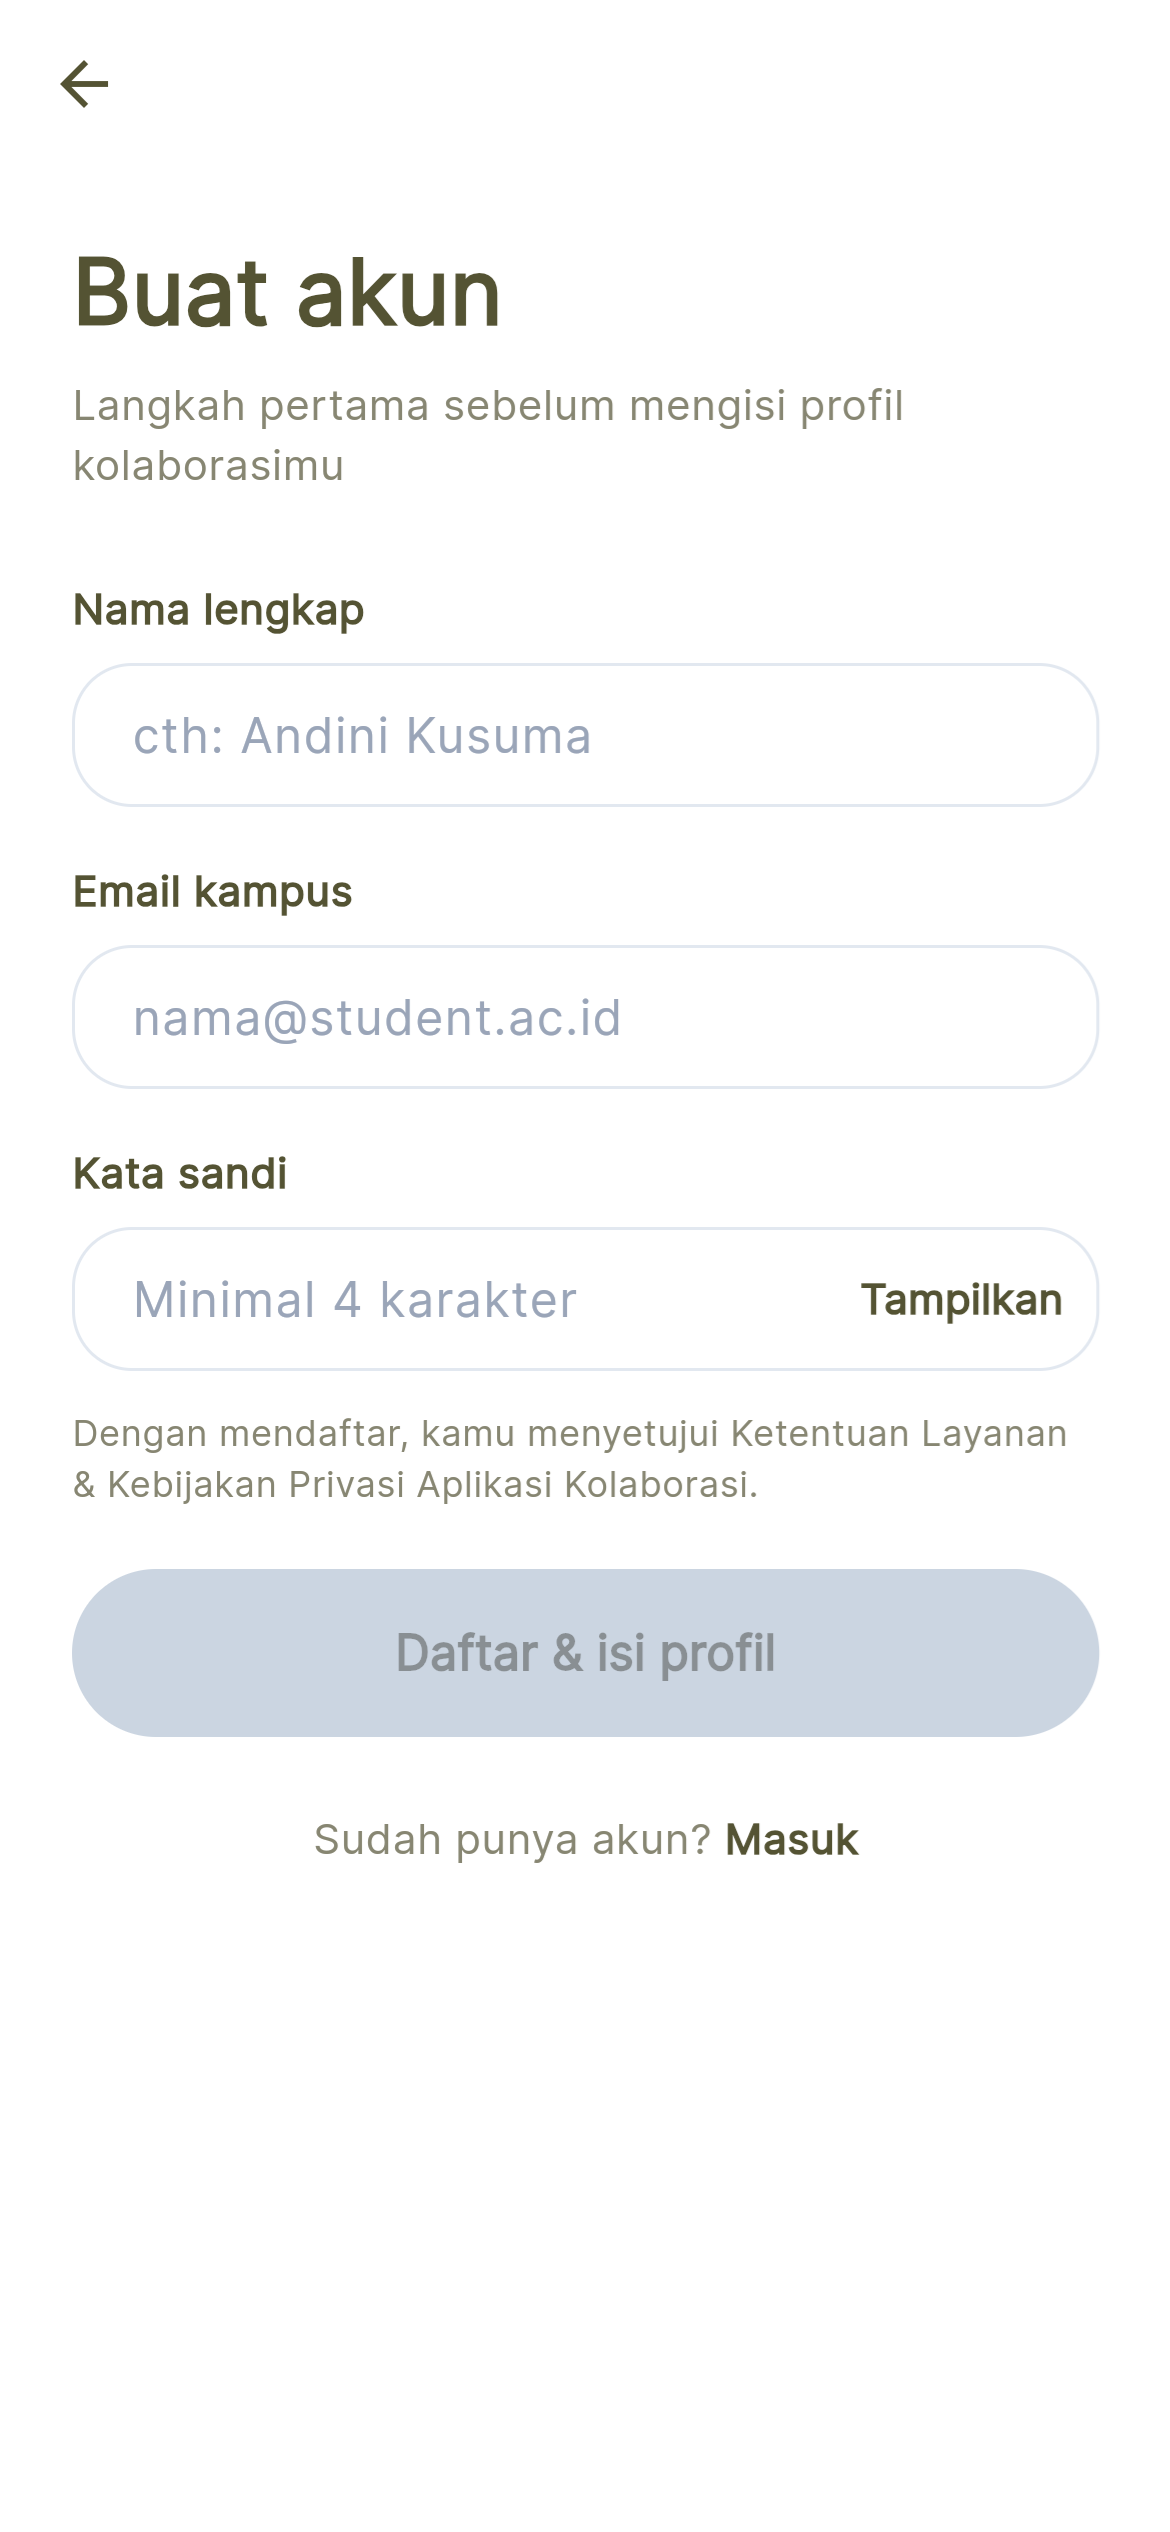
\includegraphics[width=4.5cm]{images/Layar/L1} & Formulir pengisian data akun mahasiswa baru \\
    \midrule
    L02 & 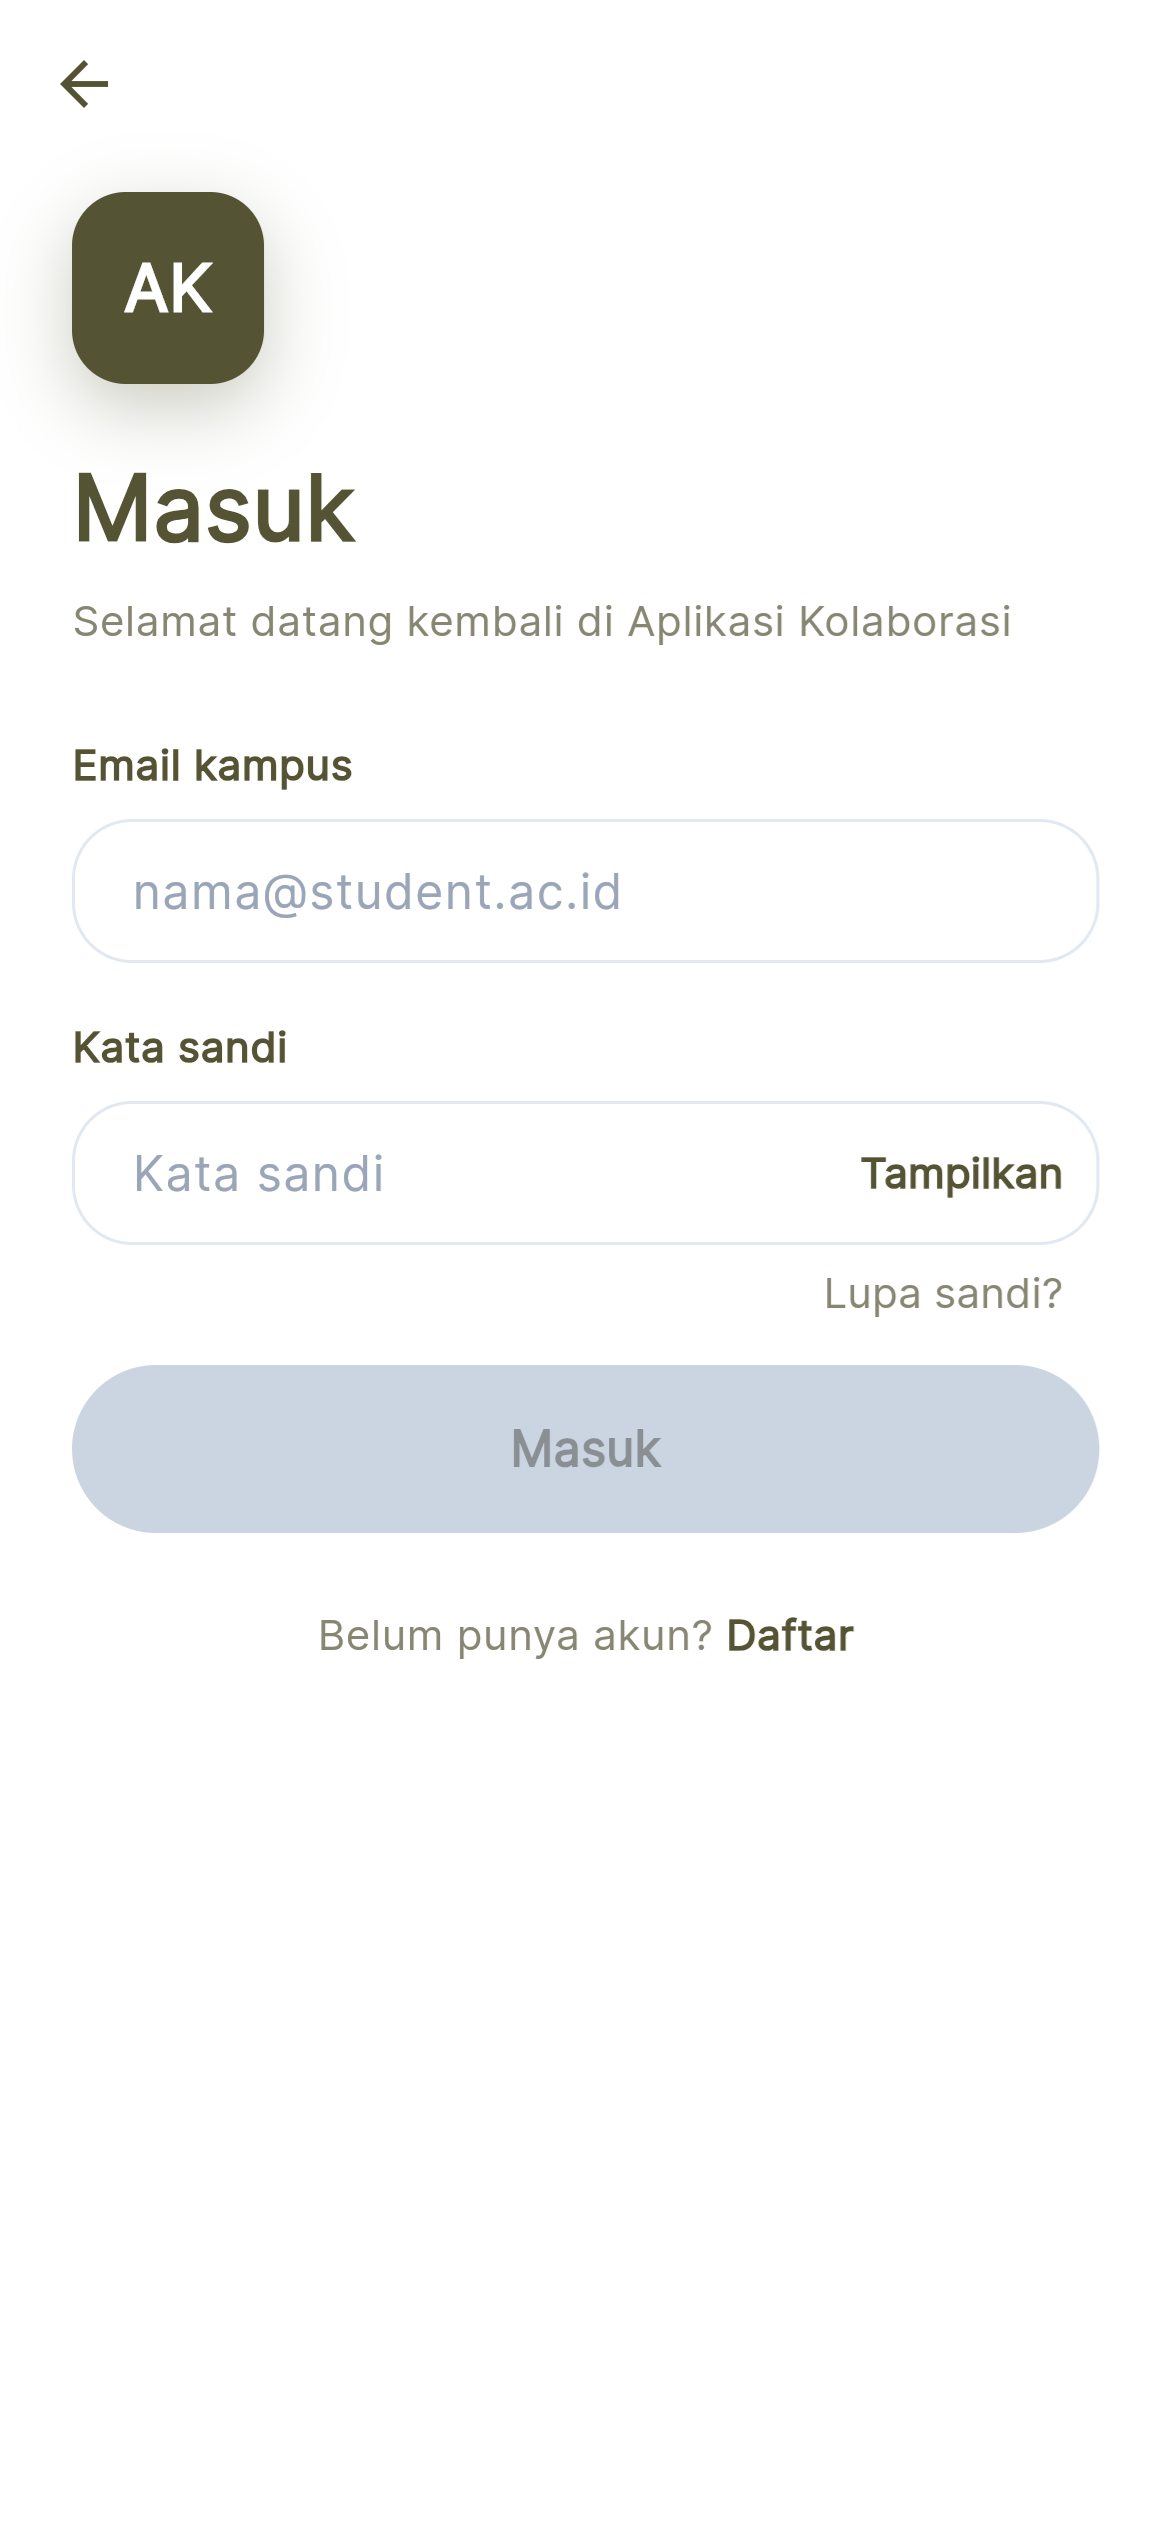
\includegraphics[width=4.5cm]{images/Layar/L2} & Formulir otentikasi menggunakan \emph{email} dan kata sandi \\
    \midrule
    L03 & 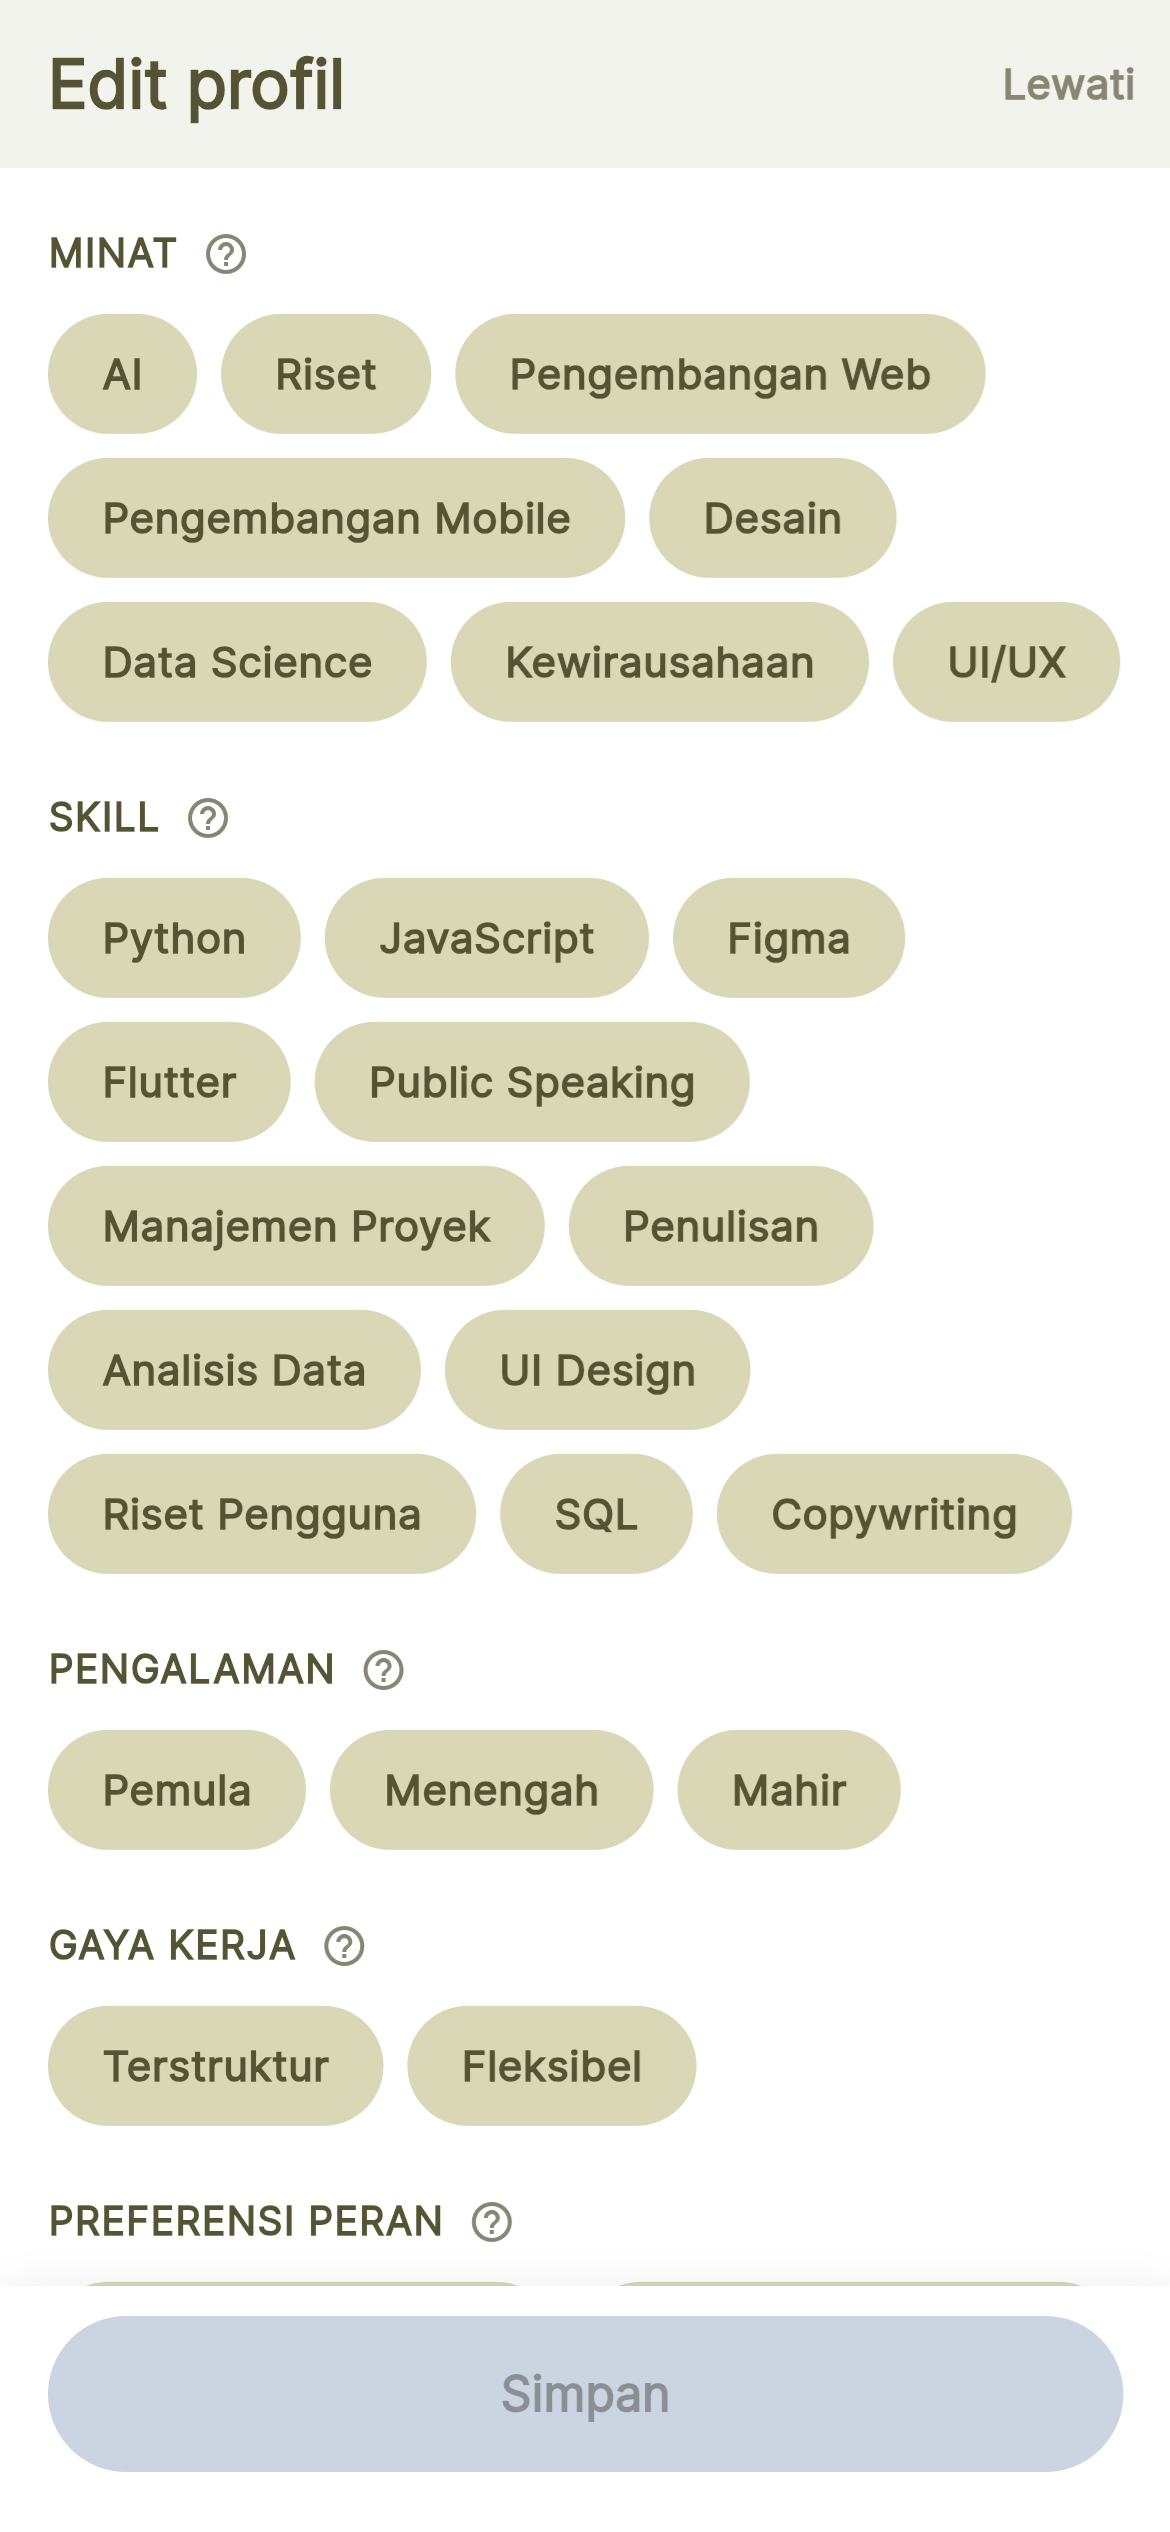
\includegraphics[width=4.5cm]{images/Layar/L3} & Halaman pengisian dan pembaruan atribut profil kolaboratif (\emph{skill}, pengalaman, minat, gaya kerja, preferensi peran) yang menjadi masukan perhitungan \emph{AffinityScore} \\
    \midrule
    L04 & 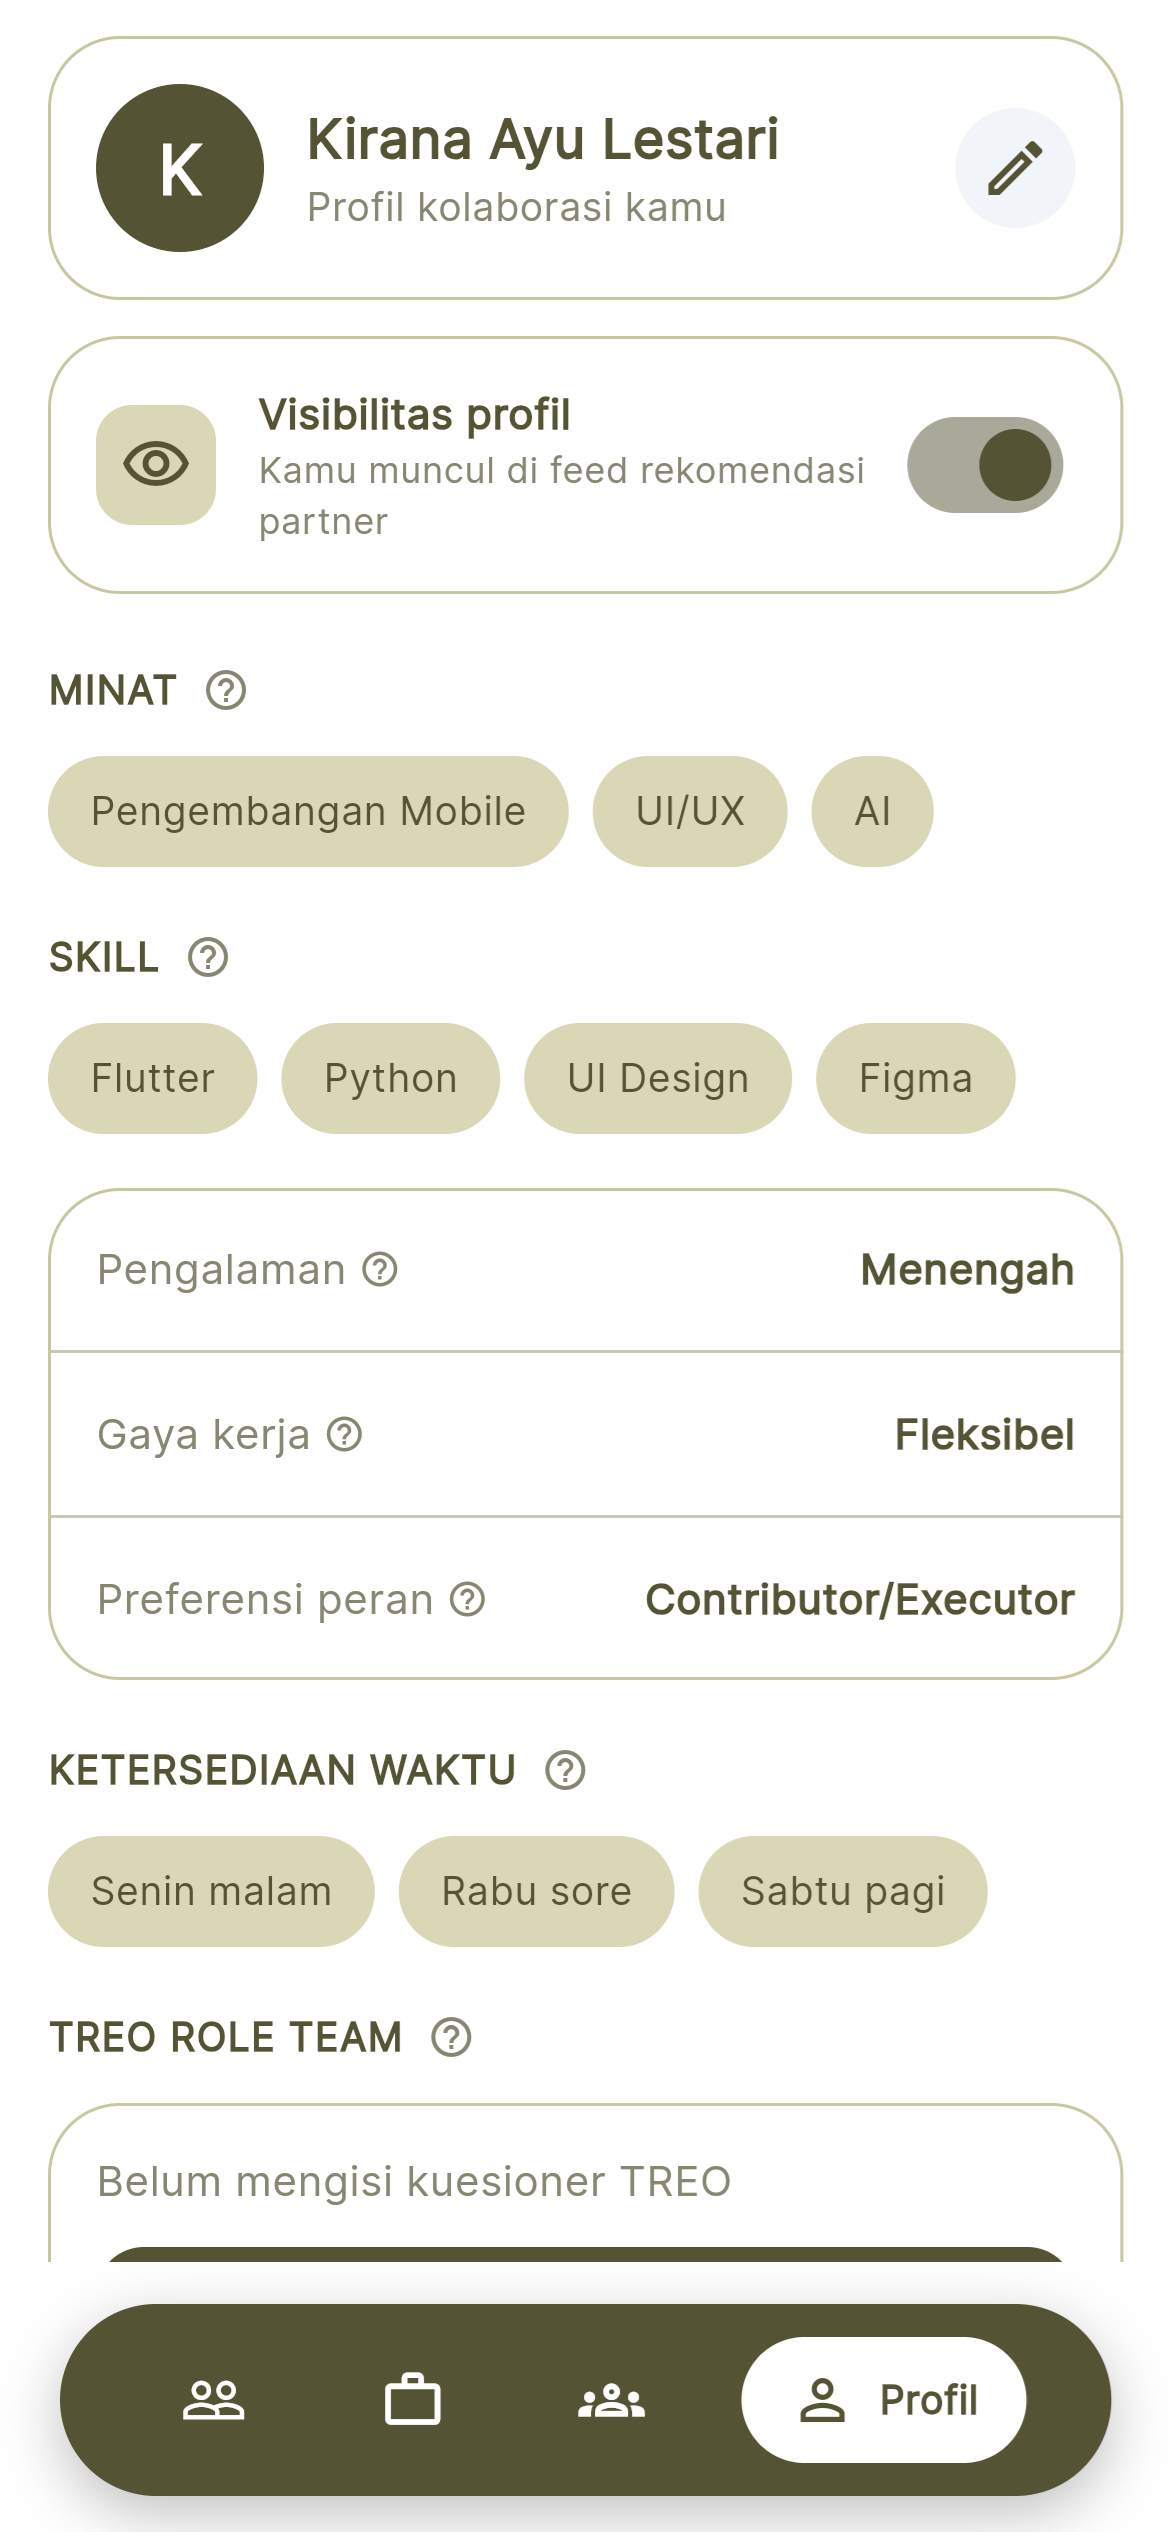
\includegraphics[width=4.5cm]{images/Layar/L4} & Menampilkan data profil pengguna serta menyediakan aksi keluar akun dan akses ke halaman pengelolaan profil \\
    \midrule
    L05 & 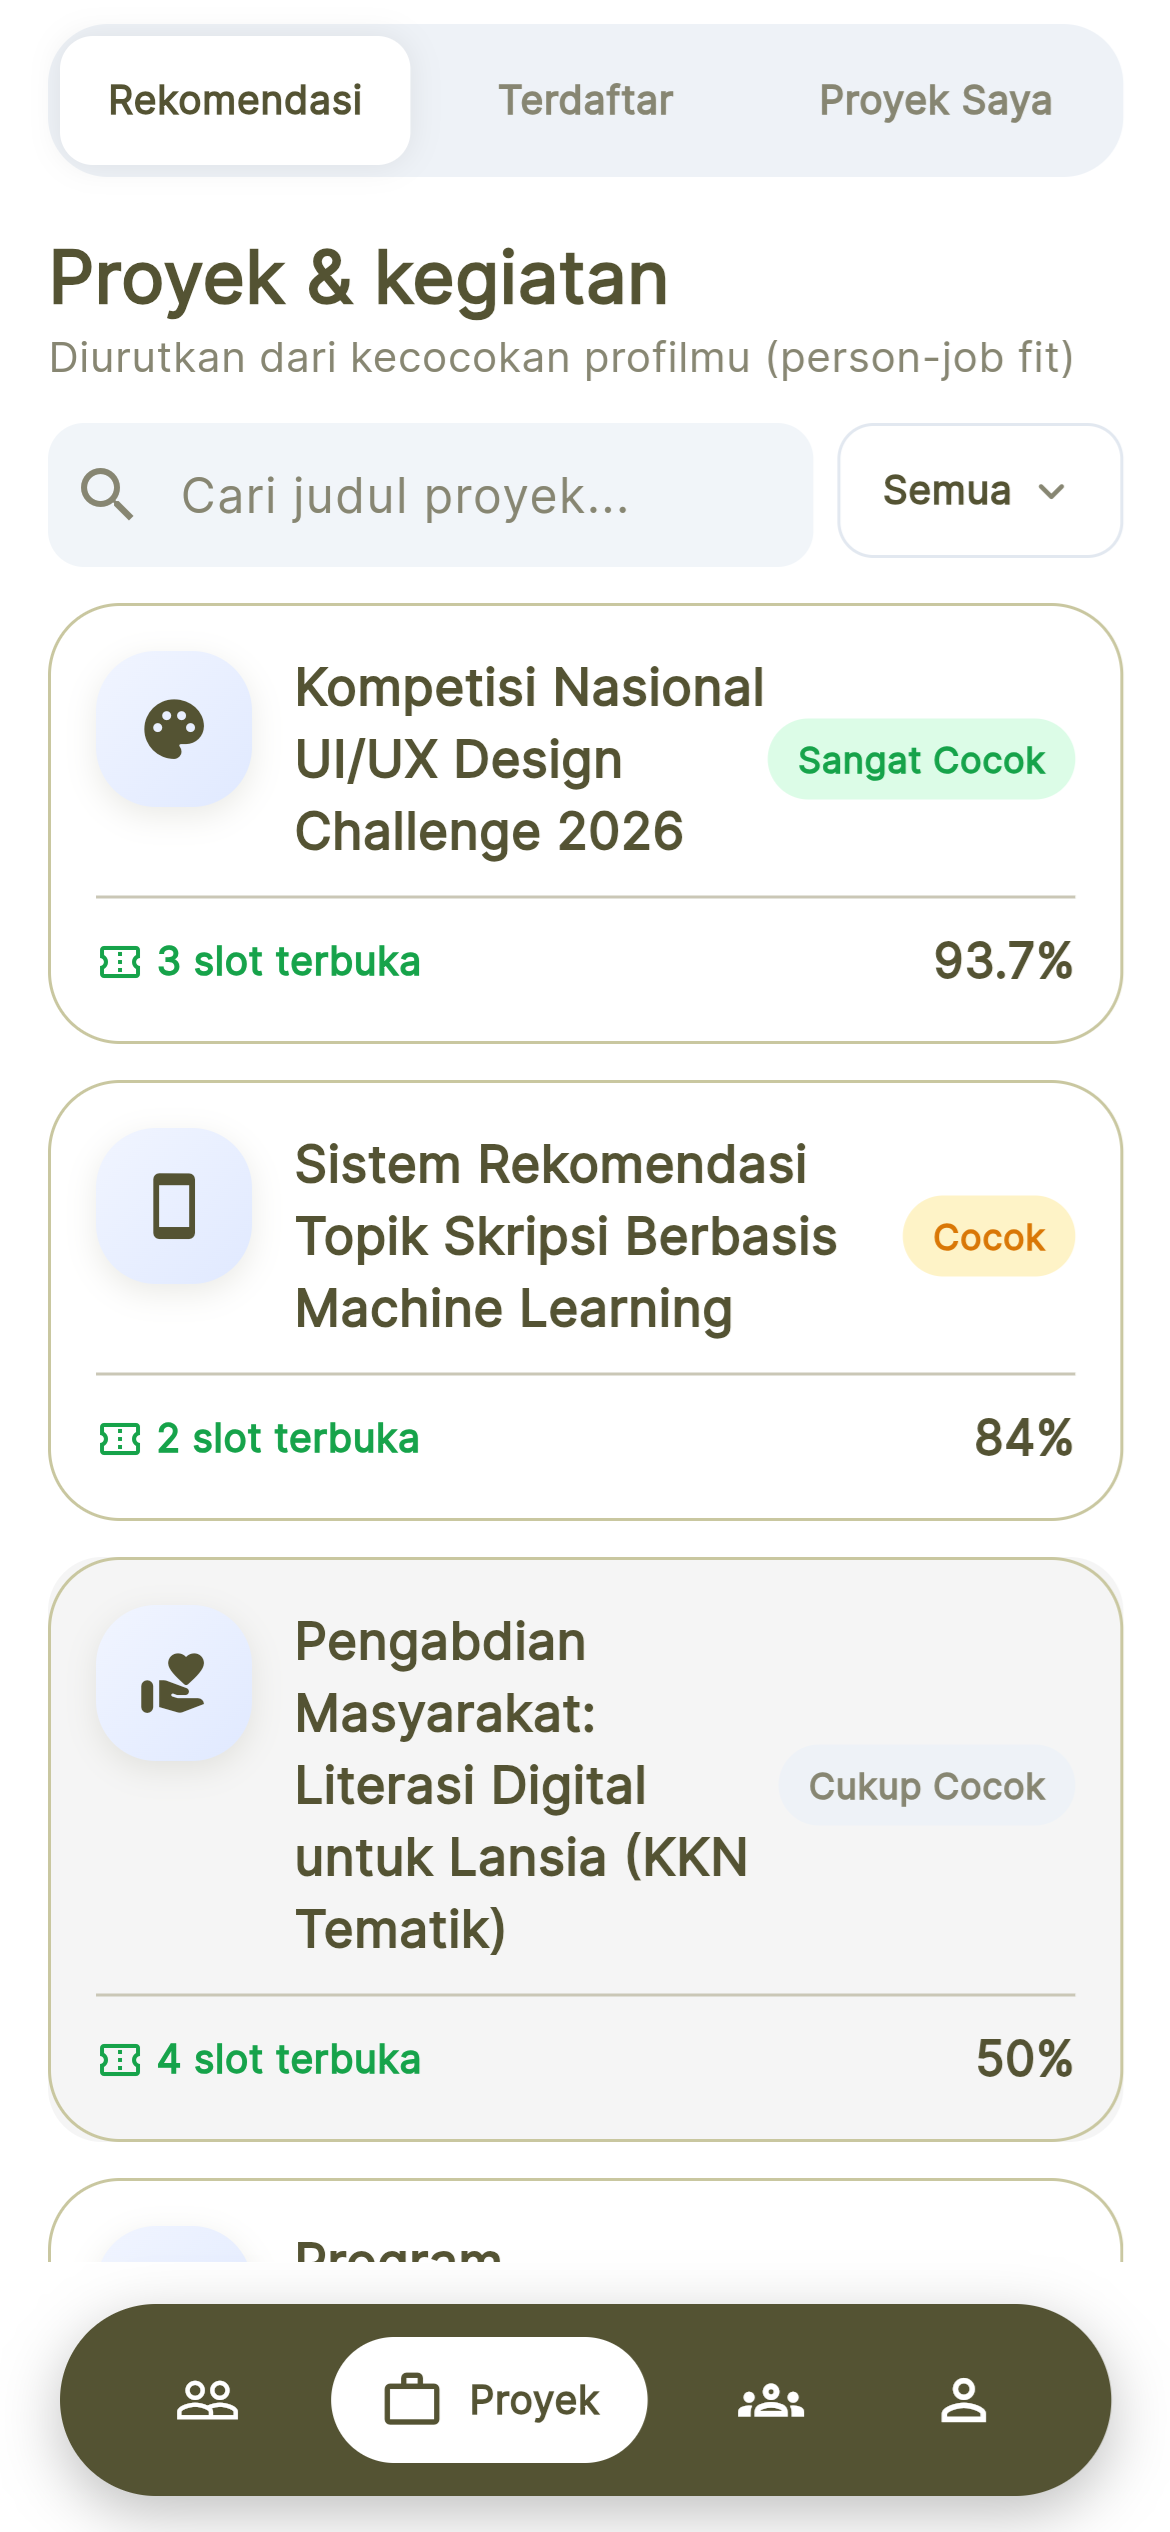
\includegraphics[width=4.5cm]{images/Layar/L5} & Menampilkan \emph{feed} kegiatan kolaboratif terurut menurun berdasarkan perhitungan \emph{AffinityScore}, dilengkapi \emph{badge} tingkat kecocokan \\
    \midrule
    L06 & 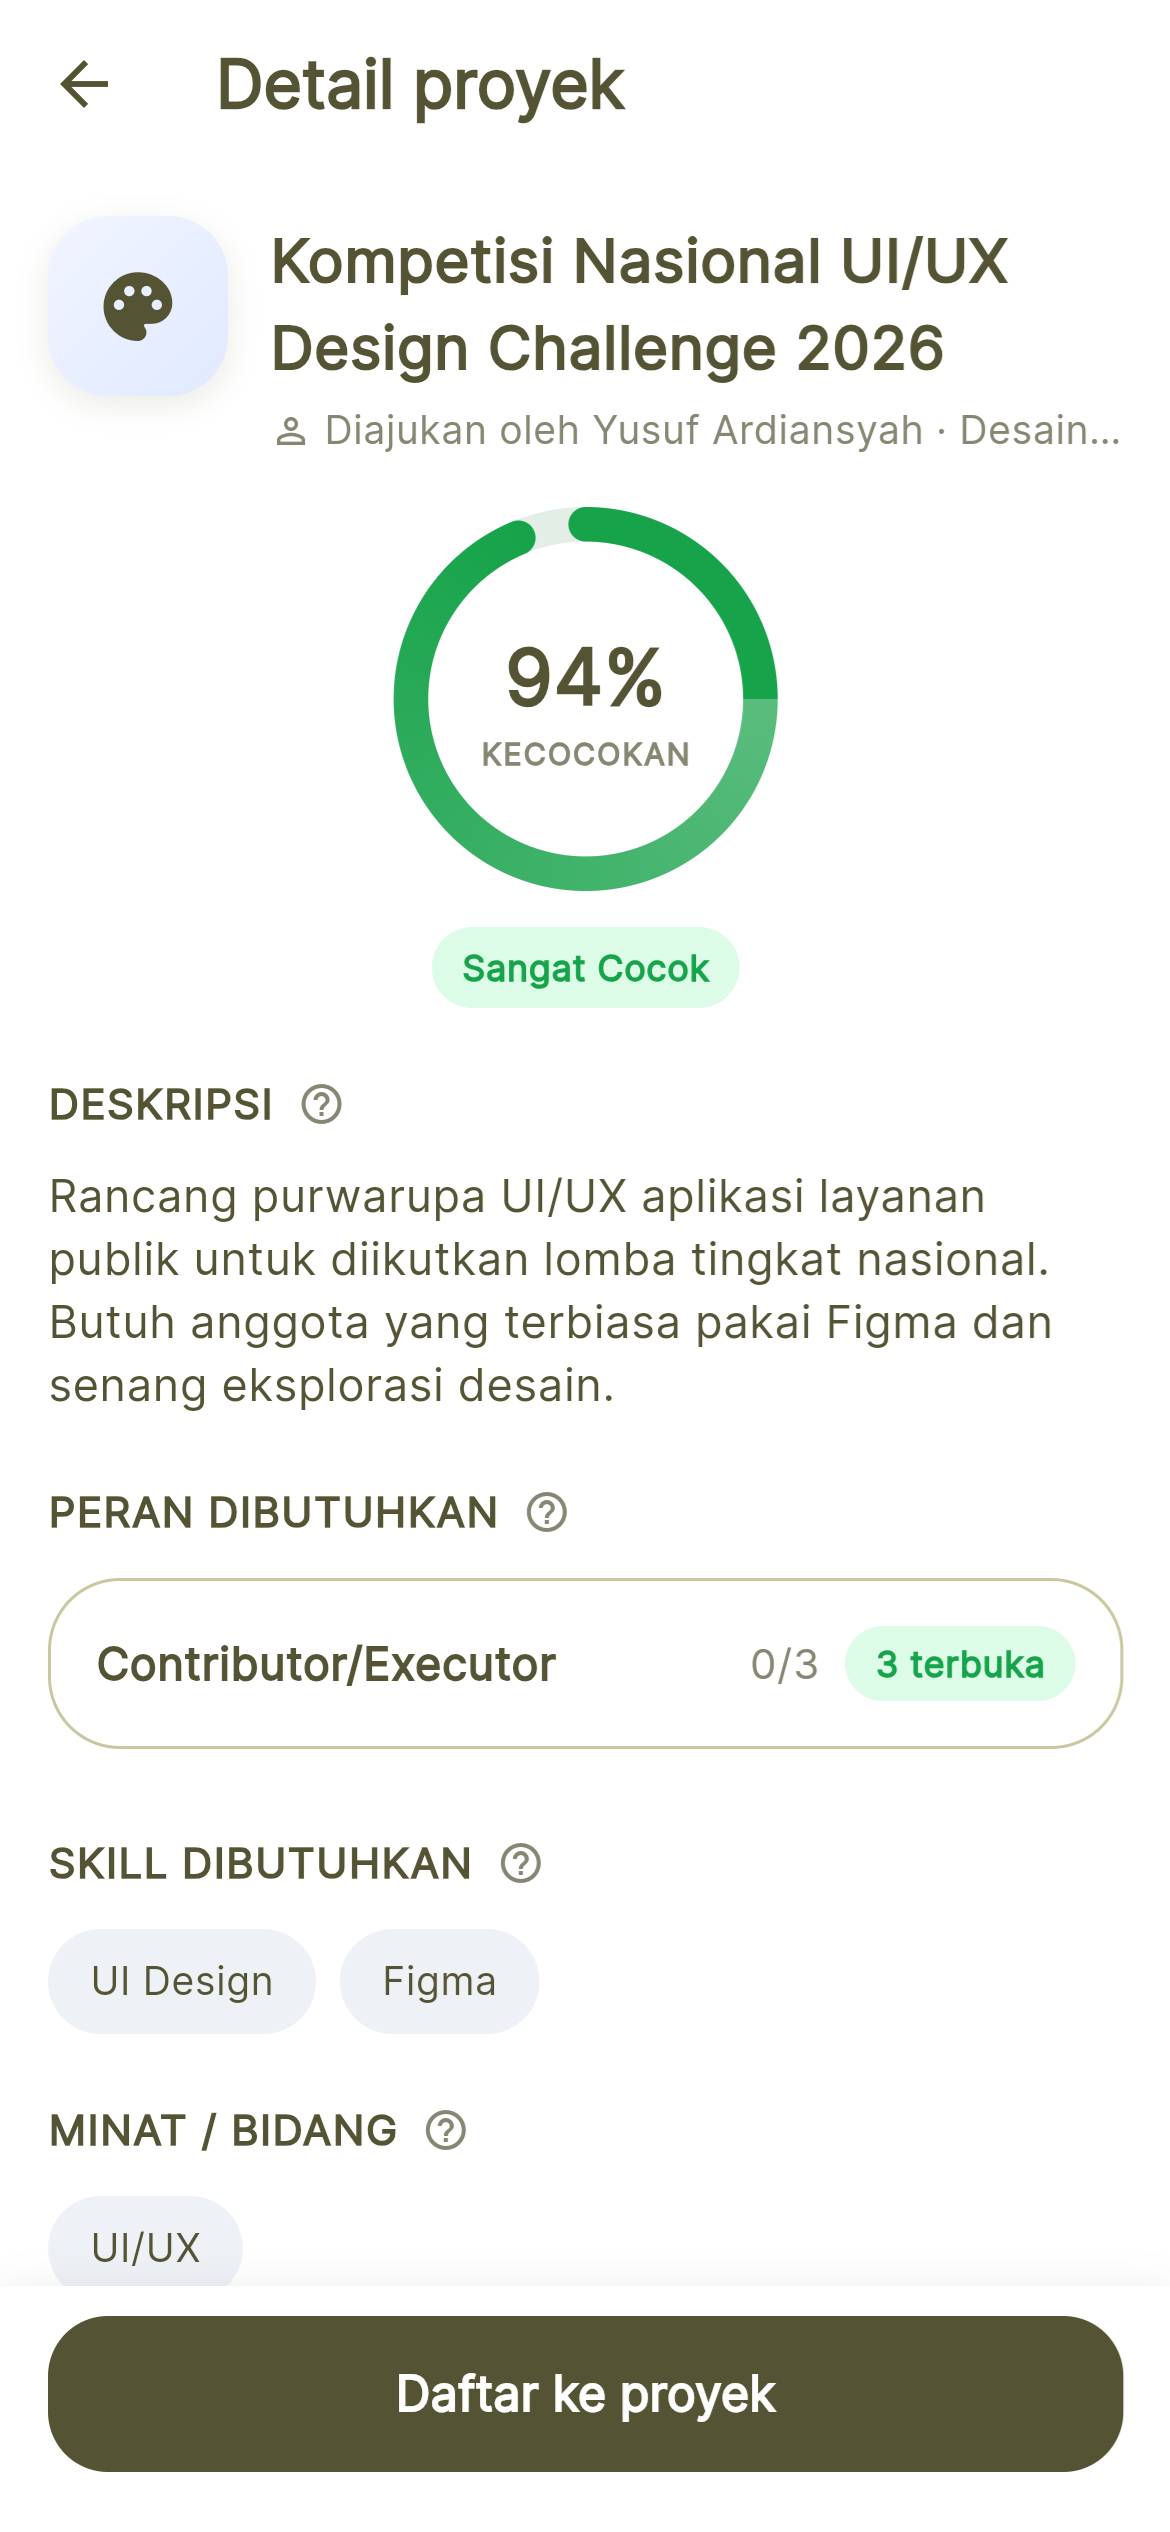
\includegraphics[width=4.5cm]{images/Layar/L6} & Menampilkan detail kegiatan kolaboratif serta menjadi titik akses untuk mengajukan pendaftaran \\
    \midrule
    L07 & 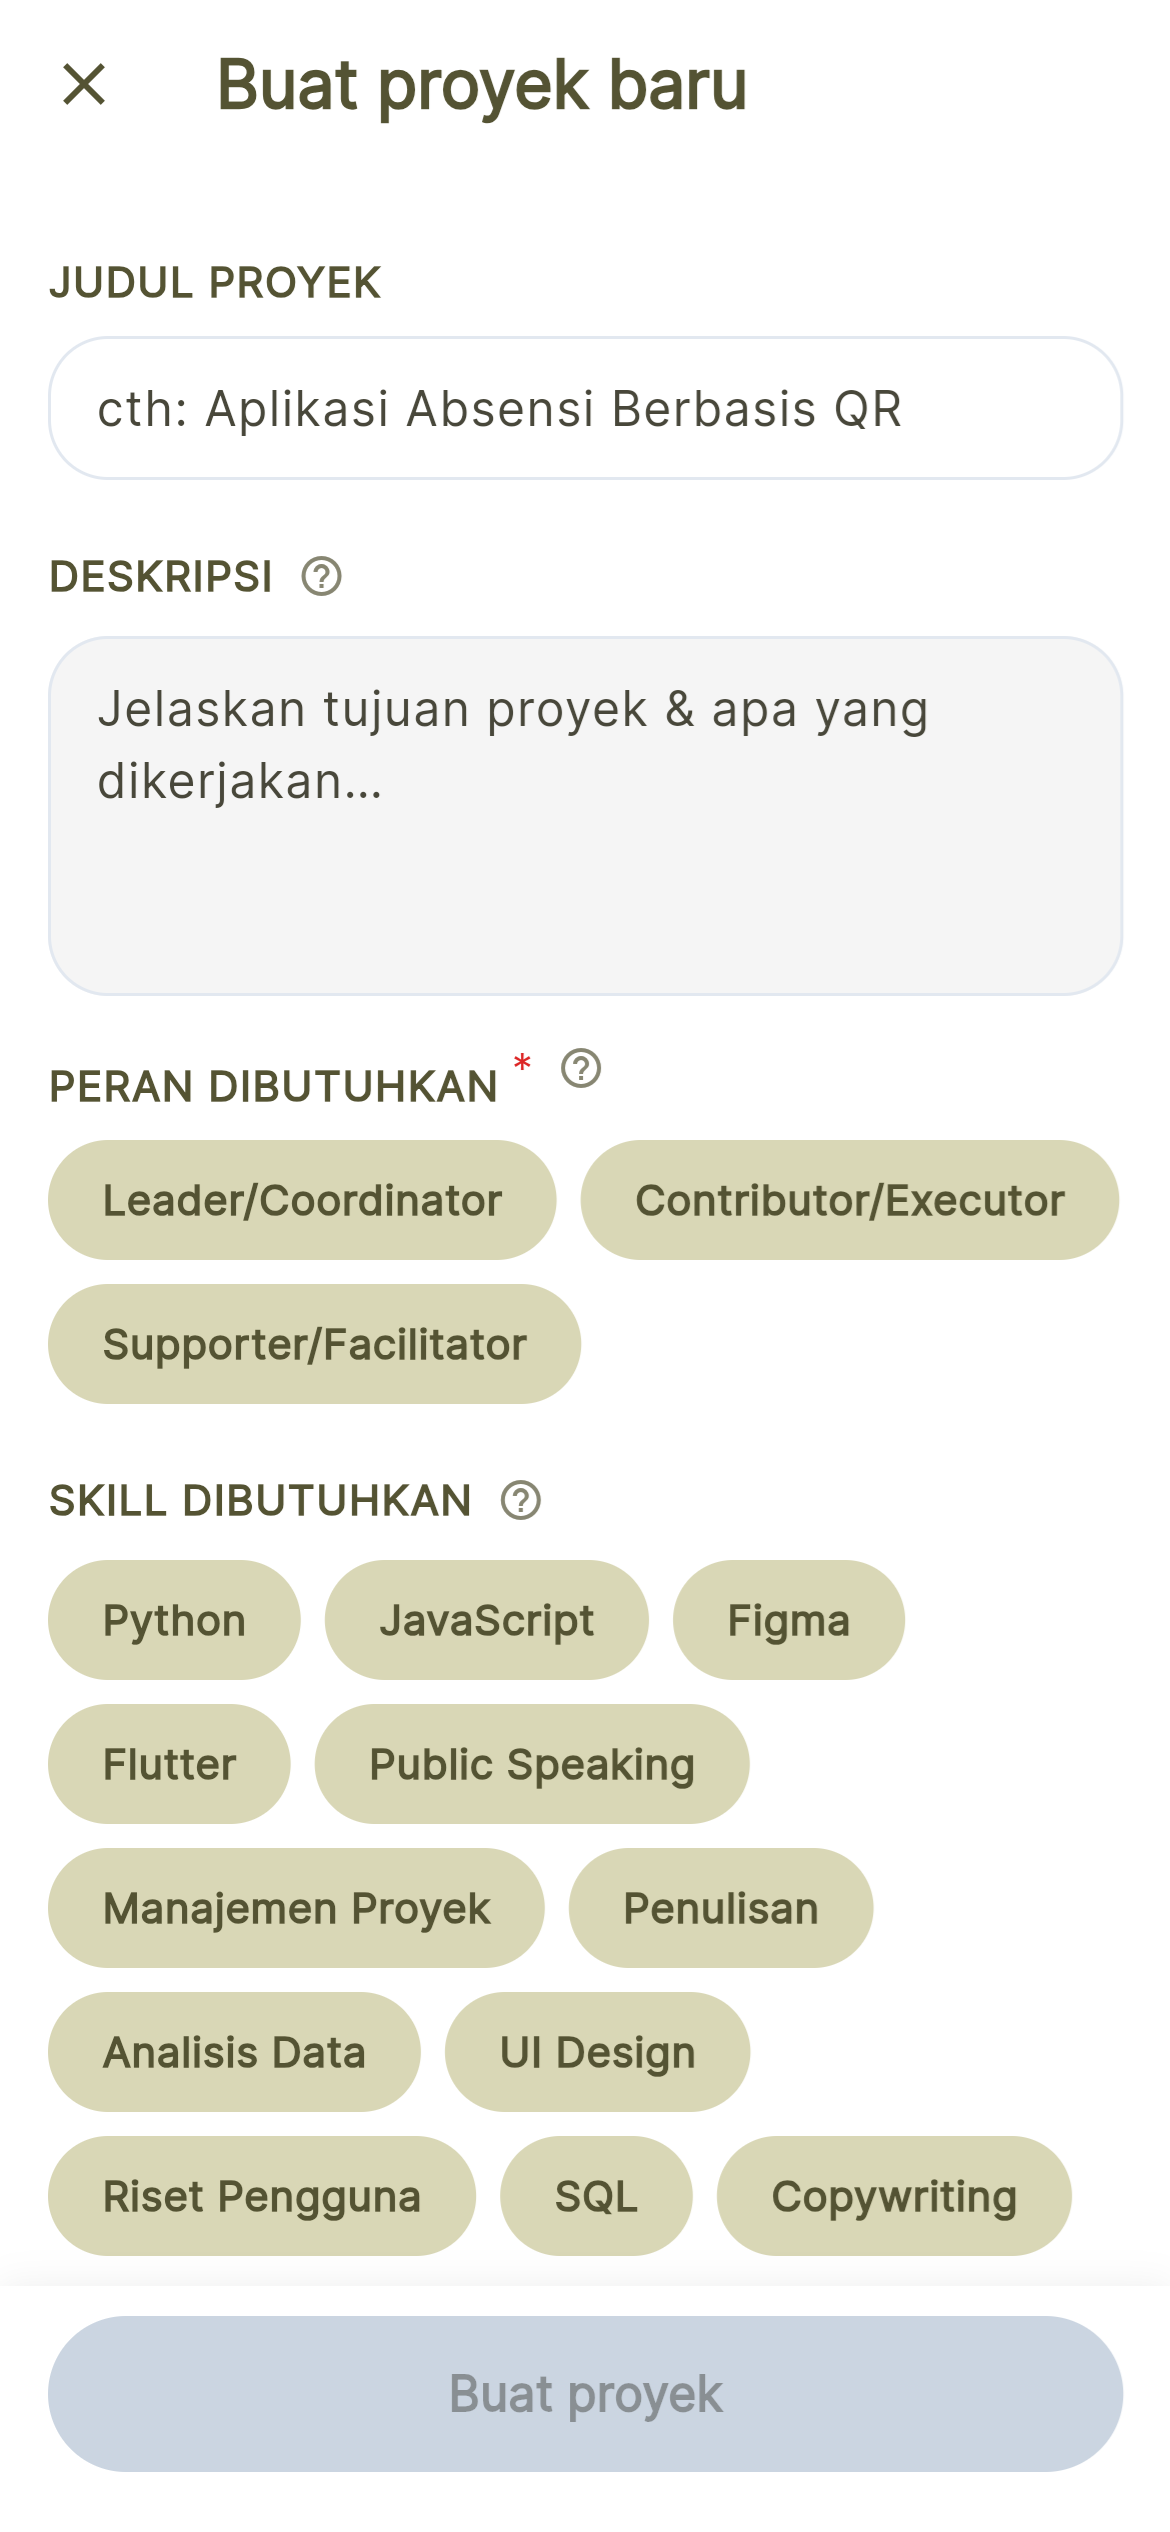
\includegraphics[width=4.5cm]{images/Layar/L7} & Formulir pembuatan kegiatan kolaboratif baru berisi judul, deskripsi, kebutuhan \emph{role} dan \emph{skill}, kuota, serta \emph{timeline} kegiatan \\
    \midrule
    L08 & 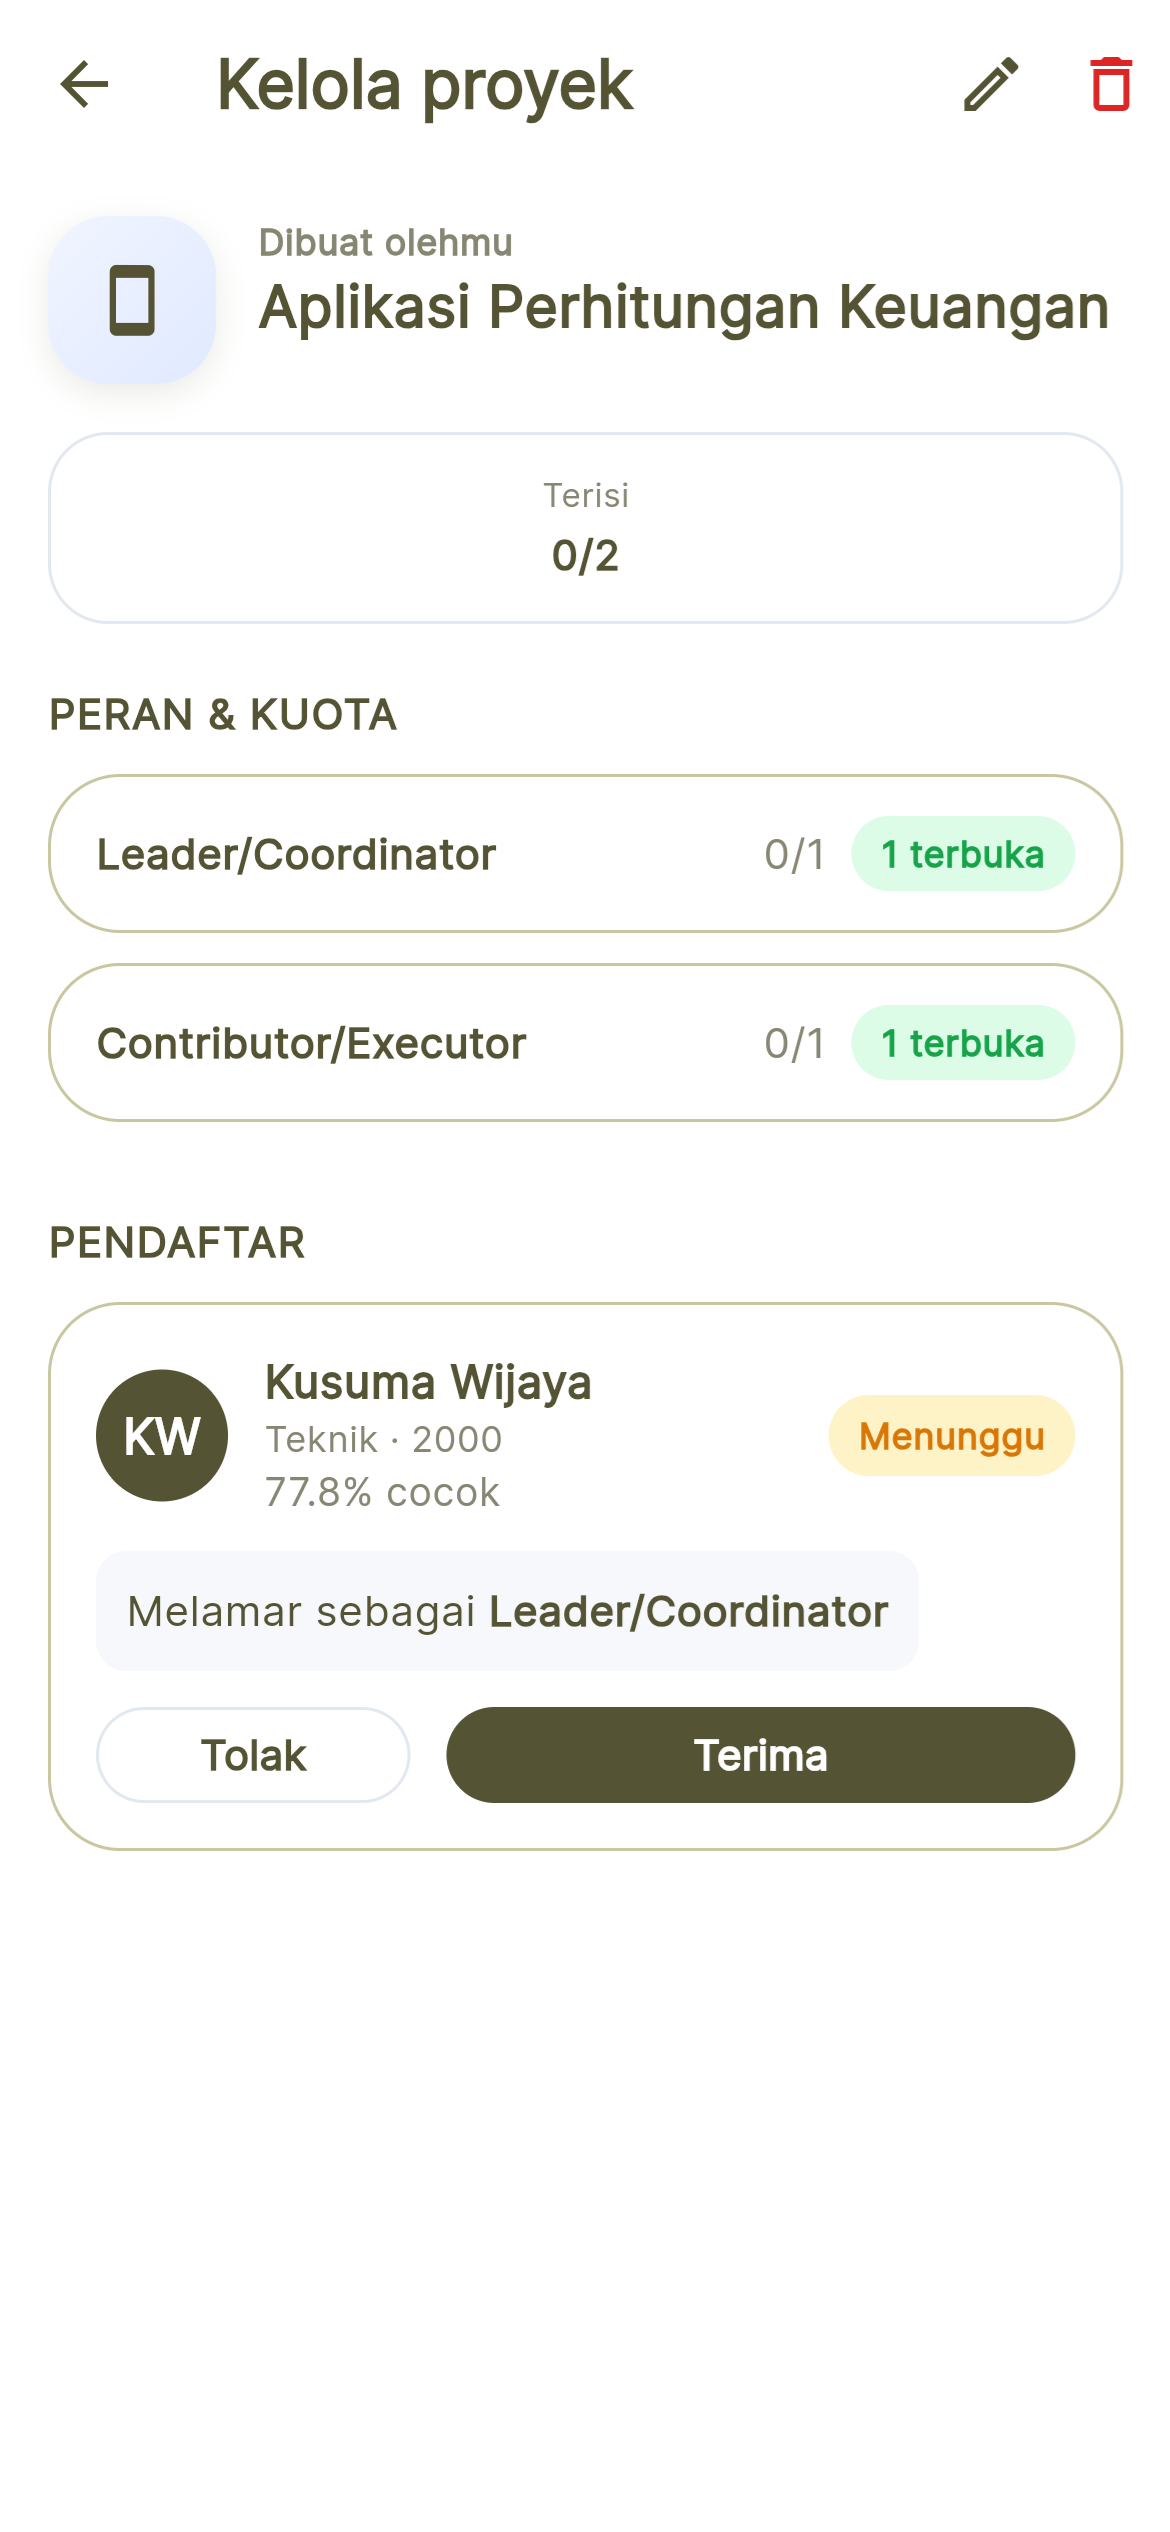
\includegraphics[width=4.5cm]{images/Layar/L8} & Menampilkan daftar pendaftar suatu kegiatan beserta \emph{role} yang dilamar, \emph{AffinityScore}, dan status pendaftaran \\
    \midrule
    L09 & 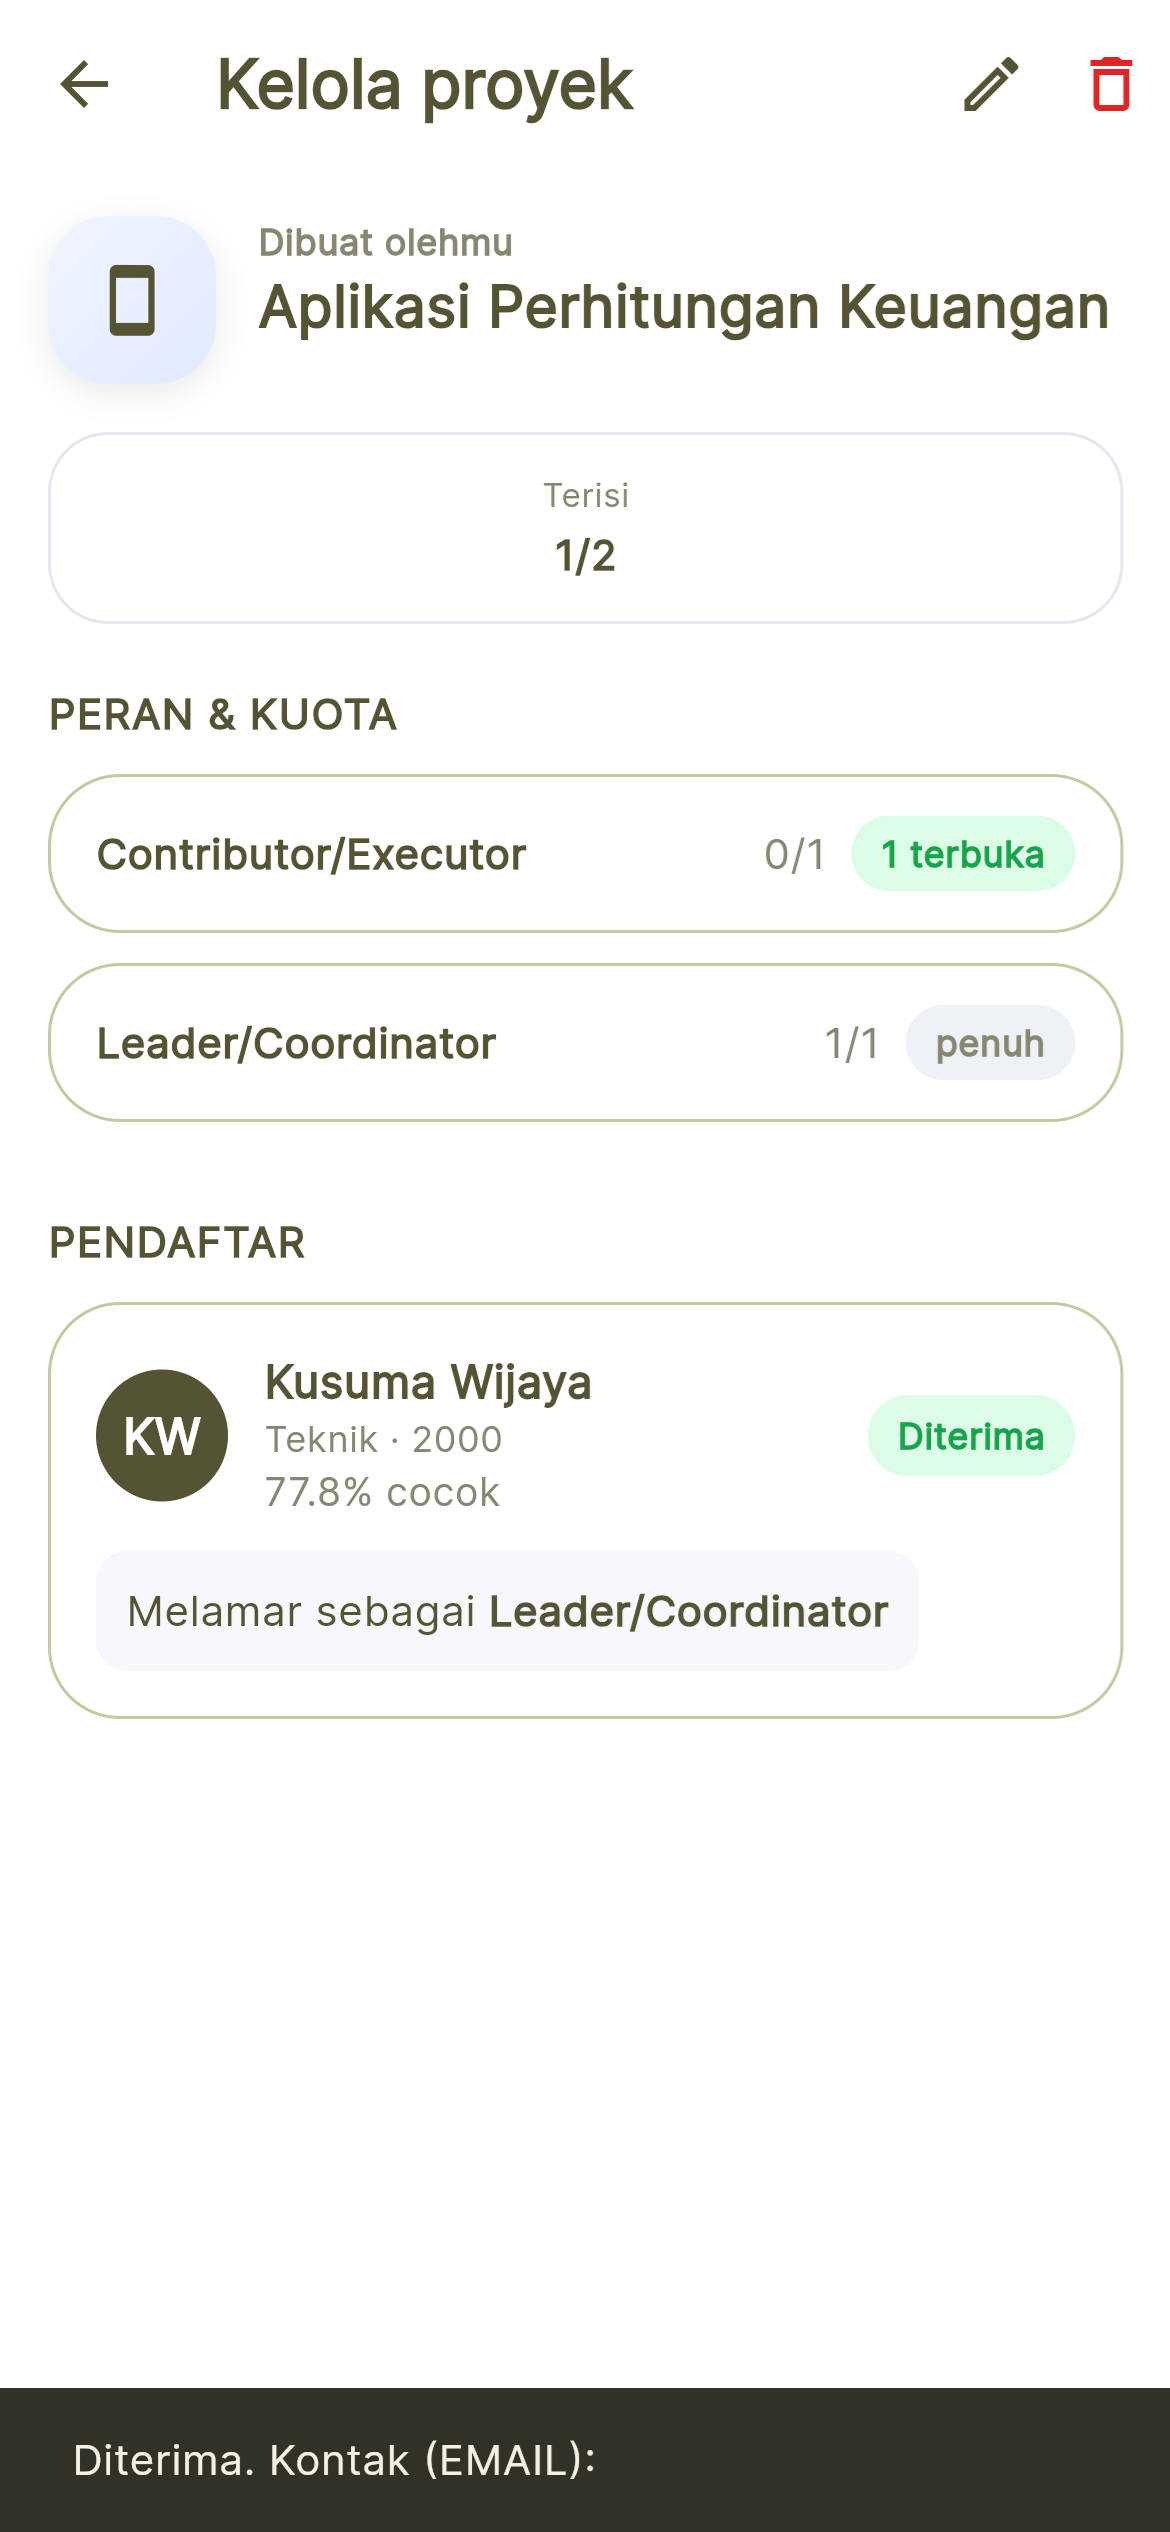
\includegraphics[width=4.5cm]{images/Layar/L9} & Antarmuka bagi pembuat kegiatan untuk meninjau, menerima, atau menolak pendaftar \\
\end{longtable}

% ==========================================
\section{Implementasi Algoritma}

Algoritma inti yang diimplementasikan pada modul \emph{People-to-Project}, sebagaimana telah dijelaskan pada subbab Perancangan Algoritma, disajikan pada Tabel~\ref{tab:algoritma-impl}.

\begin{longtable}{p{0.5cm} p{5cm} p{2.5cm} >{\raggedright\arraybackslash}p{\dimexpr\linewidth-8cm-8\tabcolsep\relax}}
  \caption{Implementasi Algoritma Modul \emph{People-to-Project}}
  \label{tab:algoritma-impl} \\
  \toprule
    \textbf{No} & \textbf{Nama Algoritma} & \textbf{Digunakan pada \emph{Use Case}} & \textbf{Nama File} \\
  \midrule
  \endfirsthead
  \multicolumn{4}{l}{\small\textit{Tabel~\ref{tab:algoritma-impl} Implementasi Algoritma Modul \emph{People-to-Project} (lanjutan)}} \\
  \toprule
    \textbf{No} & \textbf{Nama Algoritma} & \textbf{Digunakan pada \emph{Use Case}} & \textbf{Nama File} \\
  \midrule
  \endhead
  \bottomrule
  \multicolumn{4}{r}{\textit{Bersambung ke halaman berikutnya.}} \\
  \endfoot
  \bottomrule
  \endlastfoot
    1 & \emph{People-to-Project Affinity} & UC05 & \texttt{affinityProject.ts} \\
\end{longtable}

Rincian implementasi lengkap beserta kode sumber setiap fungsi \emph{AffinityEngine} disajikan pada Lampiran~\ref{chap:lampiran-b}.

% ==========================================
\section{Berkas Lain}

Berkas-berkas lain di luar berkas antarmuka yang mendukung implementasi modul \emph{People-to-Project} disajikan pada Tabel~\ref{tab:berkas-lain}.

\begin{longtable}{p{0.4cm} p{4.5cm} >{\raggedright\arraybackslash}p{\dimexpr\linewidth-4.9cm-6\tabcolsep\relax}}
  \caption{Berkas Pendukung Modul \emph{People-to-Project}}
  \label{tab:berkas-lain} \\
  \toprule
    \textbf{No} & \textbf{Nama Berkas} & \textbf{Keterangan} \\
  \midrule
  \endfirsthead
  \multicolumn{3}{l}{\small\textit{Tabel~\ref{tab:berkas-lain} Berkas Pendukung Modul \emph{People-to-Project} (lanjutan)}} \\
  \toprule
    \textbf{No} & \textbf{Nama Berkas} & \textbf{Keterangan} \\
  \midrule
  \endhead
  \bottomrule
  \multicolumn{3}{r}{\textit{Bersambung ke halaman berikutnya.}} \\
  \endfoot
  \bottomrule
  \endlastfoot
    1 & \texttt{.env} dan \texttt{.env.example} & Konfigurasi \emph{environment}, seperti kredensial basis data, \emph{port}, dan \emph{secret key}. \\
    \midrule
    2 & \texttt{prisma.ts} dan \texttt{schema.prisma} & Konfigurasi koneksi API dan basis data melalui \emph{Prisma Client} serta skema basis data. \\
    \midrule
    3 & \texttt{README.md} & Dokumentasi proyek. \\
    \midrule
    4 & \texttt{package.json} dan \texttt{package-lock.json} & Konfigurasi \emph{dependency} proyek. \\
    \midrule
    5 & \texttt{tsconfig.json} & Konfigurasi \emph{TypeScript}. \\
    \midrule
    6 & \texttt{routes.ts} dan \texttt{server.ts} & Pengaturan \emph{routing endpoint} API dan \emph{entry point} aplikasi. \\
\end{longtable}

Tautan repositori kode sumber dan berkas APK aplikasi disajikan pada Lampiran~\ref{chap:lampiran-d}.
